\documentclass[10pt,a4paper]{article}
\usepackage[margin=1.9cm]{geometry}
\usepackage[T1]{fontenc}
\usepackage{lmodern,microtype}
\usepackage{graphicx,booktabs,tabularx,array,longtable,float,caption}
\usepackage[table]{xcolor}
\usepackage{amsmath,siunitx}
\usepackage{pgfplots}
\pgfplotsset{compat=1.18}
\usepackage{tikz}
\usetikzlibrary{arrows.meta,positioning,shapes.geometric}
\usepackage{csquotes}
\usepackage[colorlinks=true,citecolor=blue!55!black,linkcolor=blue!55!black,urlcolor=blue!55!black]{hyperref}
\usepackage[backend=biber,style=ieee,sorting=none,doi=true,url=false]{biblatex}
\addbibresource{references.bib}
\definecolor{mpteal}{RGB}{20,116,135}
\definecolor{mpnavy}{RGB}{27,52,74}
\setlength{\parskip}{4pt}
\setlength{\parindent}{0pt}
\renewcommand{\arraystretch}{1.20}
\emergencystretch=3em
\title{\bfseries Laboratory and Instrumental Approaches for Measuring\\Microplastic Concentration in Surface Waters\\\large Working Principles, Evidence Map and Validation Roadmap}
\author{Y3 Group Project -- vesh sivi}
\date{October 2026}
\begin{document}
\maketitle
\begin{abstract}
This standalone draft examines laboratory reference methods and candidate monitoring instruments for microplastic (MP) concentration in river and lake \emph{surface water}. It draws on 10,833 preliminary include-candidate records from deduplicated Web of Science and Scopus exports, of which 6,654 have the overlapping Laboratory Methods label. Publication counts and title/abstract keyword frequencies characterise the literature database, not the number of experimentally validated devices. Selected source-matched papers illustrate the working principles and their limitations. The immediate engineering goal is to establish a reproducible chemistry-laboratory reference and then test whether portable instruments can predict reference MP concentrations under controlled and natural-water conditions.
\end{abstract}

\section{Dataset and interpretation}
The initial merged search contained 18,942 database records. Deduplication removed 7,318 and document-type filtering removed 727, leaving 10,897 records. Preliminary screening labelled 10,833 as include candidates and 64 for manual review. The Laboratory Methods tag covers 6,654 of the 10,833 candidates. Subcategory tags were generated by applying predefined keyword expressions to titles and abstracts within the 6,654; one record may mention multiple methods and a term mention does not confirm its use. Full-text eligibility and critical appraisal remain outstanding.

\begin{figure}[H]\centering
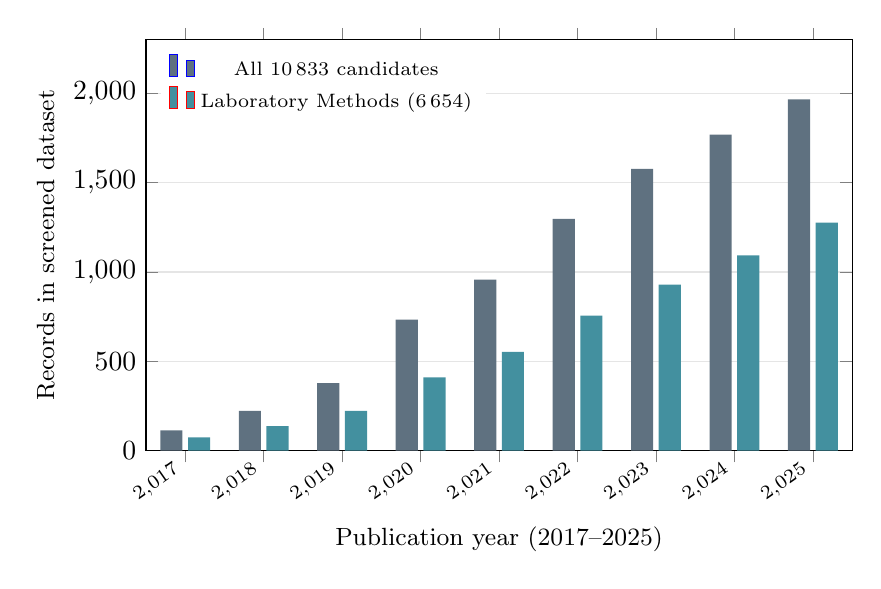
\begin{tikzpicture}
\begin{axis}[
 width=.87\linewidth,height=6.8cm,
 ybar,bar width=8pt, ymin=0, ymax=2300,
 xmin=2016.5,xmax=2025.5, xtick={2017,...,2025},
 xticklabel style={rotate=35,anchor=east,font=\scriptsize},
 ylabel={Records in screened dataset}, ylabel style={font=\small},
 xlabel={Publication year (2017--2025)},xlabel style={font=\small},
 legend style={at={(0.02,0.98)},anchor=north west,font=\scriptsize,draw=none,fill=white},
 ymajorgrids=true,grid style={gray!20},
 every axis plot/.append style={draw=none}]
\addplot+[fill=mpnavy!70] coordinates {
(2017,113)
(2018,223)
(2019,378)
(2020,733)
(2021,957)
(2022,1298)
(2023,1577)
(2024,1769)
(2025,1966)
};
\addplot+[fill=mpteal!80] coordinates {
(2017,75)
(2018,138)
(2019,222)
(2020,410)
(2021,553)
(2022,756)
(2023,930)
(2024,1093)
(2025,1277)
};
\legend{All 10\,833 candidates,Laboratory Methods (6\,654)}
\end{axis}
\end{tikzpicture}
\caption{Annual number of records \emph{within the screened dataset} (2017--2025). This is a descriptive publication trend, not a measure of method success or systematic-review inclusion. Data for 2026 are omitted to avoid partial-year comparison.}\label{fig:year}
\end{figure}

\section{What a surface-water MP measurement actually reports}
In most field surveys, a known volume of water is collected from a defined near-surface depth, retained on a filter or mesh, and analysed in the laboratory. The measurable quantity depends on \emph{particle size, sampling depth, collection volume and identification criterion}. Optical counting and spectral polymer identification can yield \emph{particles per litre}, whereas thermal analysis such as pyrolysis--GC--MS can yield \emph{polymer mass per volume}; these are different quantities and cannot be interchanged without additional size and mass information \cite{ermolin,amsterdam,pygcwater}. Small particles below the filter's effective cutoff may not be included. Surface measurements also cannot automatically represent the riverbed or the entire water column \cite{chensemenyih}.

\begin{table}[H]\centering\footnotesize
\caption{Main working principles, output quantities and expected limitations. Examples refer to studies present in the 10,833-record candidate export.}
\begin{tabularx}{\linewidth}{@{}p{2.5cm}X p{2.55cm}p{2.6cm}@{}}\toprule
Approach & Physical / chemical working principle & Typical output & Main validation concern \\ \midrule
Surface sampling + filtration & Defined volume is captured; size-based retention of particles on a membrane or net \cite{ermolin,rojas}. & Volume filtered; retained particle fraction & Representative depth, flow, mesh size, recovery \\
Microscopy / counting & Suspected particles are segmented by morphology, illumination and size \cite{narwal,unet}. & Suspected particles/L & Natural debris and observer/model false positives \\
Micro-FTIR & Infrared absorption spectrum is matched against polymer spectra \cite{ftirraman,fan}. & Polymer-confirmed count, type, size (within method range) & Small-particle identification, spectra quality \\
Raman & Inelastic laser scattering identifies chemical fingerprints \cite{ftirraman,ramanspiked}. & Polymer type; confirmed particles & Fluorescence, matrix effects, time per particle \\
Pyrolysis--GC--MS & Thermal breakdown products identify and quantify polymers by mass \cite{amsterdam,pygcwater}. & Polymer mass per volume & Particle number and size generally not measured \\
Fluorescence imaging & Fluorescent stain enhances visual contrast of particles \cite{nilered}. & Fluorescent suspected particle count & Non-specific staining; confirmation needed \\
Polarised scattering & Polarisation-resolved particle-scattered light measures optical features \cite{polarized}. & Particle optical signatures & Sediment/algae discrimination and range \\
RGB / remote imagery & Image-derived water features are linked through a model to lab reference values \cite{aerial,chenlangat}. & Calibrated prediction, if validated & No direct polymer identification; site dependence \\
\bottomrule\end{tabularx}\label{tab:methods}
\end{table}

\section{Research-method frequencies}
Figure~\ref{fig:methods} and Table~\ref{tab:freq} show the full set of fourteen categories in the previously generated Laboratory Methods classification. They are \emph{title/abstract keyword matches} among 6,654 candidate papers. Counts overlap and should not be used as evidence of equipment adoption, accuracy or comparative effectiveness.

\begin{figure}[H]\centering
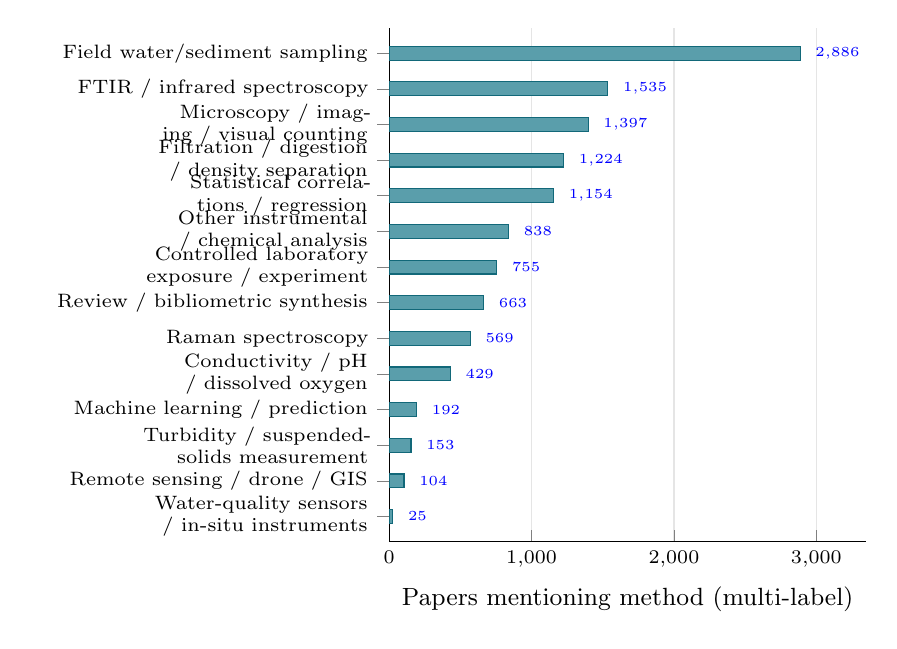
\begin{tikzpicture}
\begin{axis}[
 xbar, bar width=5pt,width=.63\linewidth,height=8.1cm,
 xmin=0,xmax=3350,ymin=-.7,ymax=13.7,
 ytick={0,...,13},yticklabels={
{Water-quality sensors / in-situ instruments},
{Remote sensing / drone / GIS},
{Turbidity / suspended-solids measurement},
{Machine learning / prediction},
{Conductivity / pH / dissolved oxygen},
{Raman spectroscopy},
{Review / bibliometric synthesis},
{Controlled laboratory exposure / experiment},
{Other instrumental / chemical analysis},
{Statistical correlations / regression},
{Filtration / digestion / density separation},
{Microscopy / imaging / visual counting},
{FTIR / infrared spectroscopy},
{Field water/sediment sampling}
 },
 yticklabel style={font=\scriptsize,align=right,text width=4.2cm},
 tick label style={font=\scriptsize},
 xlabel={Papers mentioning method (multi-label)},xlabel style={font=\small},
 axis x line*=bottom,axis y line*=left,
 xmajorgrids=true,grid style={gray!20},
 nodes near coords,point meta=x,
 every node near coord/.append style={font=\tiny,anchor=west,xshift=2pt}
]
\addplot+[draw=mpteal!90!black,fill=mpteal!70] coordinates {
(25,0)
(104,1)
(153,2)
(192,3)
(429,4)
(569,5)
(663,6)
(755,7)
(838,8)
(1154,9)
(1224,10)
(1397,11)
(1535,12)
(2886,13)
};
\end{axis}
\end{tikzpicture}
\caption{Automatically tagged laboratory-method keywords in the Laboratory Methods subset ($n=6{,}654$); not confirmed study procedures.}\label{fig:methods}
\end{figure}

\begin{table}[H]\centering\small
\caption{All defined Laboratory Methods categories in the abstract-screened subset.}\label{tab:freq}
\begin{tabularx}{\linewidth}{@{}Xrr@{}}\toprule
Category & Mentions & Share of 6,654 \\ \midrule
Field water/sediment sampling & 2,886 & 43.4\% \\
FTIR / infrared spectroscopy & 1,535 & 23.1\% \\
Microscopy / imaging / visual counting & 1,397 & 21.0\% \\
Filtration / digestion / density separation & 1,224 & 18.4\% \\
Statistical correlations / regression & 1,154 & 17.3\% \\
Other instrumental / chemical analysis & 838 & 12.6\% \\
Controlled laboratory exposure / experiment & 755 & 11.3\% \\
Review / bibliometric synthesis & 663 & 10.0\% \\
Raman spectroscopy & 569 & 8.6\% \\
Conductivity / pH / dissolved oxygen & 429 & 6.4\% \\
Machine learning / prediction & 192 & 2.9\% \\
Turbidity / suspended-solids measurement & 153 & 2.3\% \\
Remote sensing / drone / GIS & 104 & 1.6\% \\
Water-quality sensors / in-situ instruments & 25 & 0.4\% \\
\bottomrule\end{tabularx}
\end{table}

\section{Representative findings relevant to equipment selection}
\begin{table}[H]\centering\scriptsize
\caption{Selected studies in the original 10,833 candidates: procedures and results reported in their abstracts. Values are source-specific, not a pooled estimate; full-text verification remains necessary.}\label{tab:studies}
\begin{tabularx}{\linewidth}{@{}p{2.4cm} X X@{}}\toprule
Study and context & Reported method / principle & Reported outcome and relevance \\ \midrule
Odora et al. (2024), Balu River \cite{odora} & Six near-surface sampling sites; stereomicroscopy and FTIR. & Mean $102.5\pm12.83$ items/L; variations among locations reinforce the need for spatial reference samples. \\
Rojas-Luna et al. (2023), Luruaco Lake \cite{rojas} & 72 samples across dry/rainy campaigns; peroxide digestion, NaCl density separation and filtration. & Abundance 0--3.83 particles/L; sampling period and preparation affect comparison. \\
Chen et al. (2021), Langat River \cite{chenlangat} & 508 water samples over 12 months at eight sites; discharge and suspended-sediment associations. & Mean 4.39 particles/L; observed sediment/discharge relationships suggest \emph{testing} turbidity as a proxy, not assuming it works everywhere. \\
Chen et al. (2023), Semenyih River \cite{chensemenyih} & Replicate river-water and riverbed samples at eight sites over three dates. & Water mean $3.12\pm2.49$ particles/L; sediment results differed spatially, so surface-only monitoring has defined limits. \\
Amsterdam canals study (2024) \cite{amsterdam} & Surface-water pump in the 10--300 $\mu$m fraction; micro-FTIR imaging versus pyrolysis--GC--MS. & 16--107 particles/m$^3$ in sampled size range; showed why count and mass measurement are complementary. \\
Raman spiking study (2024) \cite{ramanspiked} & Known plastic nanoparticles spiked into artificial and environmental fresh/saltwater; Raman analysis. & Detection limits depended on particle properties and water matrix; informs matrix-interference testing. \\
Liu et al. (2021) \cite{polarized} & Polarisation of light scattered at 120$^\circ$; machine-learning classification. & Demonstrated discrimination using test particles, algae and natural-water samples; feasibility is not field-calibrated concentration accuracy. \\
Lee et al. (2022) \cite{unet} & U-Net neural-network segmentation and post-processing of microscope images. & Reported human-level counting in cluttered images; still requires labelled data and chemical confirmation. \\
\bottomrule\end{tabularx}
\end{table}

\section{Selecting the laboratory reference and field device}
\textbf{Reference measurement.} A chemistry laboratory can establish a reproducible particle-concentration reference by sampling a known water volume, retaining a specified size fraction, using contamination-controlled preparation, counting candidate particles and spectrally confirming polymer identity on a defensible sampling or subsampling basis \cite{ermolin,ftirraman,qc}. Where polymer mass rather than number is central, pyrolysis--GC--MS provides a complementary chemical-mass reference rather than an interchangeable count \cite{amsterdam,pygcwater}.

\textbf{Portable device.} Turbidity or RGB signals are mainly sensitive to \emph{all} optical scatterers, including mineral sediment and organic matter. Conductivity reflects dissolved ions and therefore does not specifically identify plastic particles. A correlation with microplastic concentration must be established from \emph{paired} laboratory measurements, with independent tests under varied matrix conditions. The Langat River study reported an observational association of MP counts with suspended sediments, while controlled flume evidence indicates that suspended sediments can also change where fibres reside in the water column \cite{chenlangat,turbidity}. No universal turbidity--MP or conductivity--MP conversion is established by the screened counts.

\begin{figure}[H]\centering
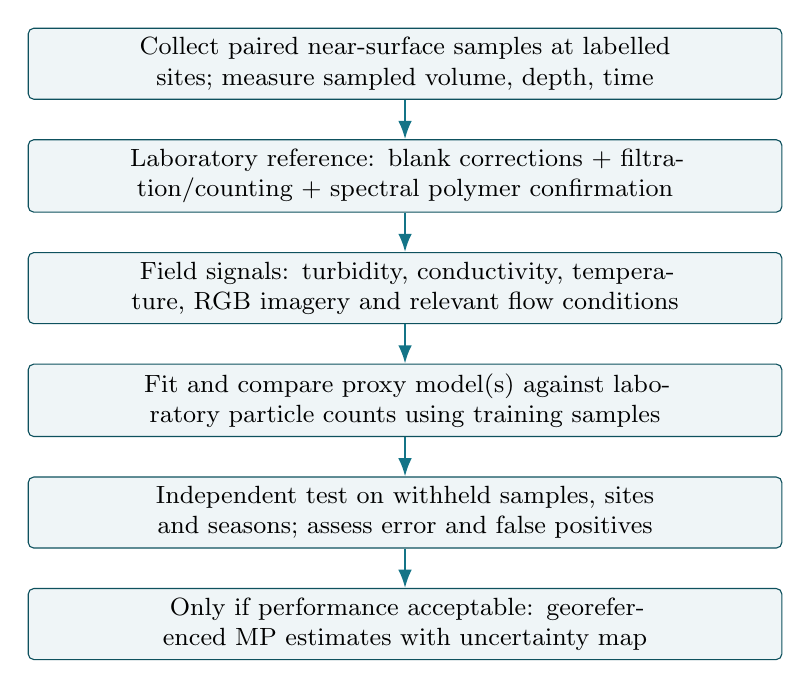
\begin{tikzpicture}[>=Latex, node distance=5mm,
 n/.style={draw=mpteal!70!black,fill=mpteal!7,rounded corners=2pt,text width=.77\linewidth,align=center,minimum height=9mm,font=\small},
 a/.style={->,thick,draw=mpteal}]
\node[n] (s) {Collect paired near-surface samples at labelled sites; measure sampled volume, depth, time};
\node[n,below=of s] (r) {Laboratory reference: blank corrections + filtration/counting + spectral polymer confirmation};
\node[n,below=of r] (f) {Field signals: turbidity, conductivity, temperature, RGB imagery and relevant flow conditions};
\node[n,below=of f] (c) {Fit and compare proxy model(s) against laboratory particle counts using training samples};
\node[n,below=of c] (v) {Independent test on withheld samples, sites and seasons; assess error and false positives};
\node[n,below=of v] (m) {Only if performance acceptable: georeferenced MP estimates with uncertainty map};
\foreach \u/\v in {s/r,r/f,f/c,c/v,v/m}{\draw[a] (\u)--(\v);}
\end{tikzpicture}
\caption{Proposed test-and-validation chain for the Year 3 project. This is an engineering plan, not a result established by the screened literature.}\label{fig:validation}
\end{figure}

\begin{table}[H]\centering\footnotesize
\caption{Proposed controlled-sample matrix to discuss with the chemistry laboratory. The entries are design recommendations, not previously validated operating concentrations.}\label{tab:labplan}
\begin{tabularx}{\linewidth}{@{}p{2.65cm} X X@{}}\toprule
Test material & Purpose & Measurement / success criterion \\ \midrule
Filtered-water blank and procedural blank & Identify lab-air, container and reagent contamination & Blank-corrected particle counts; document contamination events \\
Known MP particle spikes at multiple levels & Establish response over measurable range & Measured versus independently verified particles/L and recovery \\
Different particle sizes, shapes and polymers & Test dependence on material properties & Per-group false negatives and counting error \\
Non-plastic sediment/algae without MPs & Challenge optical specificity & False-positive signal against clean reference \\
Mixed MPs + sediment at variable turbidity & Assess matrix interference & Error relative to matched reference MP count \\
Salinity/ionic-strength and pH perturbations & Challenge conductivity / resistivity proxy & Verify whether apparent signal tracks ions instead of MPs \\
Independent natural river-water campaigns & Out-of-sample generalisation & MAE/RMSE, bias, site-to-site stability, confidence limits \\
\bottomrule\end{tabularx}
\end{table}

For a particle-count reference, use a fixed sampling volume $V$ (L), polymer-confirmed count $N_{\rm MP}$, adjusted blank contribution $N_{\rm blank}$, and a separately estimated recovery fraction $r$ when justified:
\begin{equation}
 C_{\rm ref}\,(\mathrm{particles/L}) = \frac{N_{\rm MP}-N_{\rm blank}}{V\,r}.
\end{equation}
Record the lower size limit, sample depth, blank adjustment and any recovery correction explicitly. If $r$ has not been measured, report uncorrected concentrations and recovery uncertainty rather than assuming $r=1$.

\textbf{Decision gate.} Begin with \emph{laboratory reference feasibility} (instrument access, size limit, available polymer standards, blank/recovery controls), then a \emph{small controlled pilot}, then \emph{paired river samples}. If a low-cost turbidity/conductivity model cannot predict polymer-confirmed MP counts robustly, change to a direct particle-detection or sample-concentration architecture rather than reporting proxy values as MP concentration.

\section{Limitations and immediate next steps}
This is a \emph{preliminary abstract-based evidence map}. The 6,654 method-tagged records have not been confirmed as using the method, and the selected papers are illustrative rather than an exhaustive systematic synthesis. Before final thesis claims, inspect full texts for sampling depth, size cutoff, analytical blanks, recovery, polymer confirmation and uncertainty. Arrange a chemistry-lab meeting to select the reference endpoint (particles/L, optionally mass/L), source characterised reference MP particles, define a feasible sampling/filtration volume, and conduct blinded replicate tests.

\printbibliography[title={References}]
\end{document}
